%! TEX program = xelatex
%! TEX root = ../root.tex

\section{实验原理}
\subsection{Datapath}
为了支持多周期操作本实验对数据通路进行了修改,想要成功完成此次实验,对Datapath的熟练掌握自然是必要的。
下面就是本次实验所参照的Datapath

\begin{figure}[H] %H为当前位置,!htb为忽略美学标准,htbp为浮动图形
	\centering %图片居中
	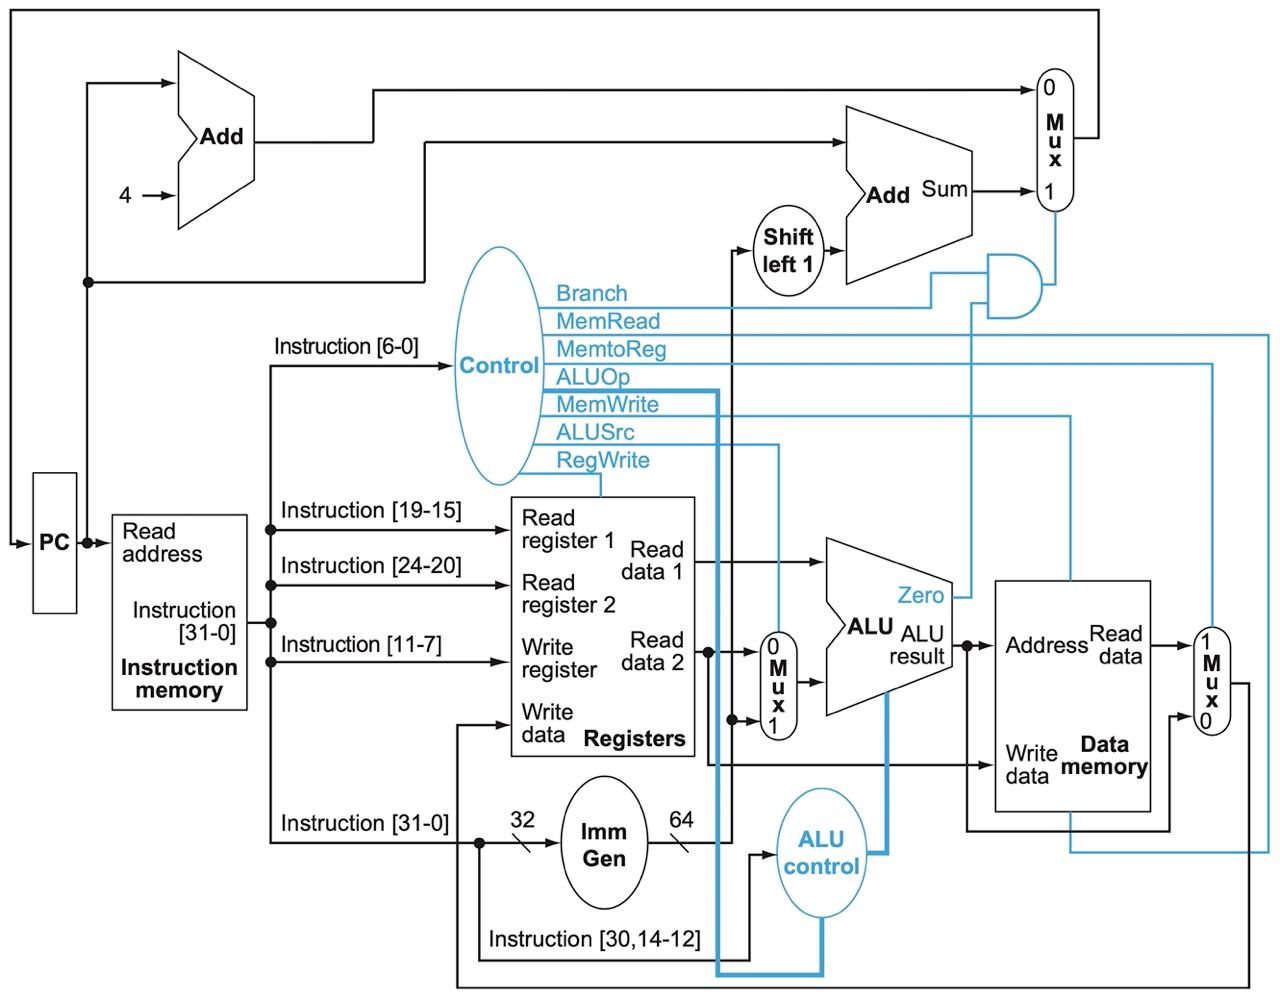
\includegraphics[width=1.0\textwidth]{figs/datapath.png} %插入图片,[]中设置图片大小,{}中是图片文件名
	\caption{Datapath} %最终文档中希望显示的图片标题
	\label{Fig.1} %用于文内引用的标签
\end{figure}
CMU模块安置在流水线的MEM阶段,其与CPU之间有一系列的接口,包括Data\_Read,Data\_Write,Address等,这提供了CPU与cache之间数据传输的通道。同时,CMU还与Memory之间有一系列接口,以用于cache和memory之间进行数据传输。
\subsection{Cache Operation Flow}
CMU中的操作流程如下图所示
\begin{figure}[H] %H为当前位置,!htb为忽略美学标准,htbp为浮动图形
	\centering %图片居中
	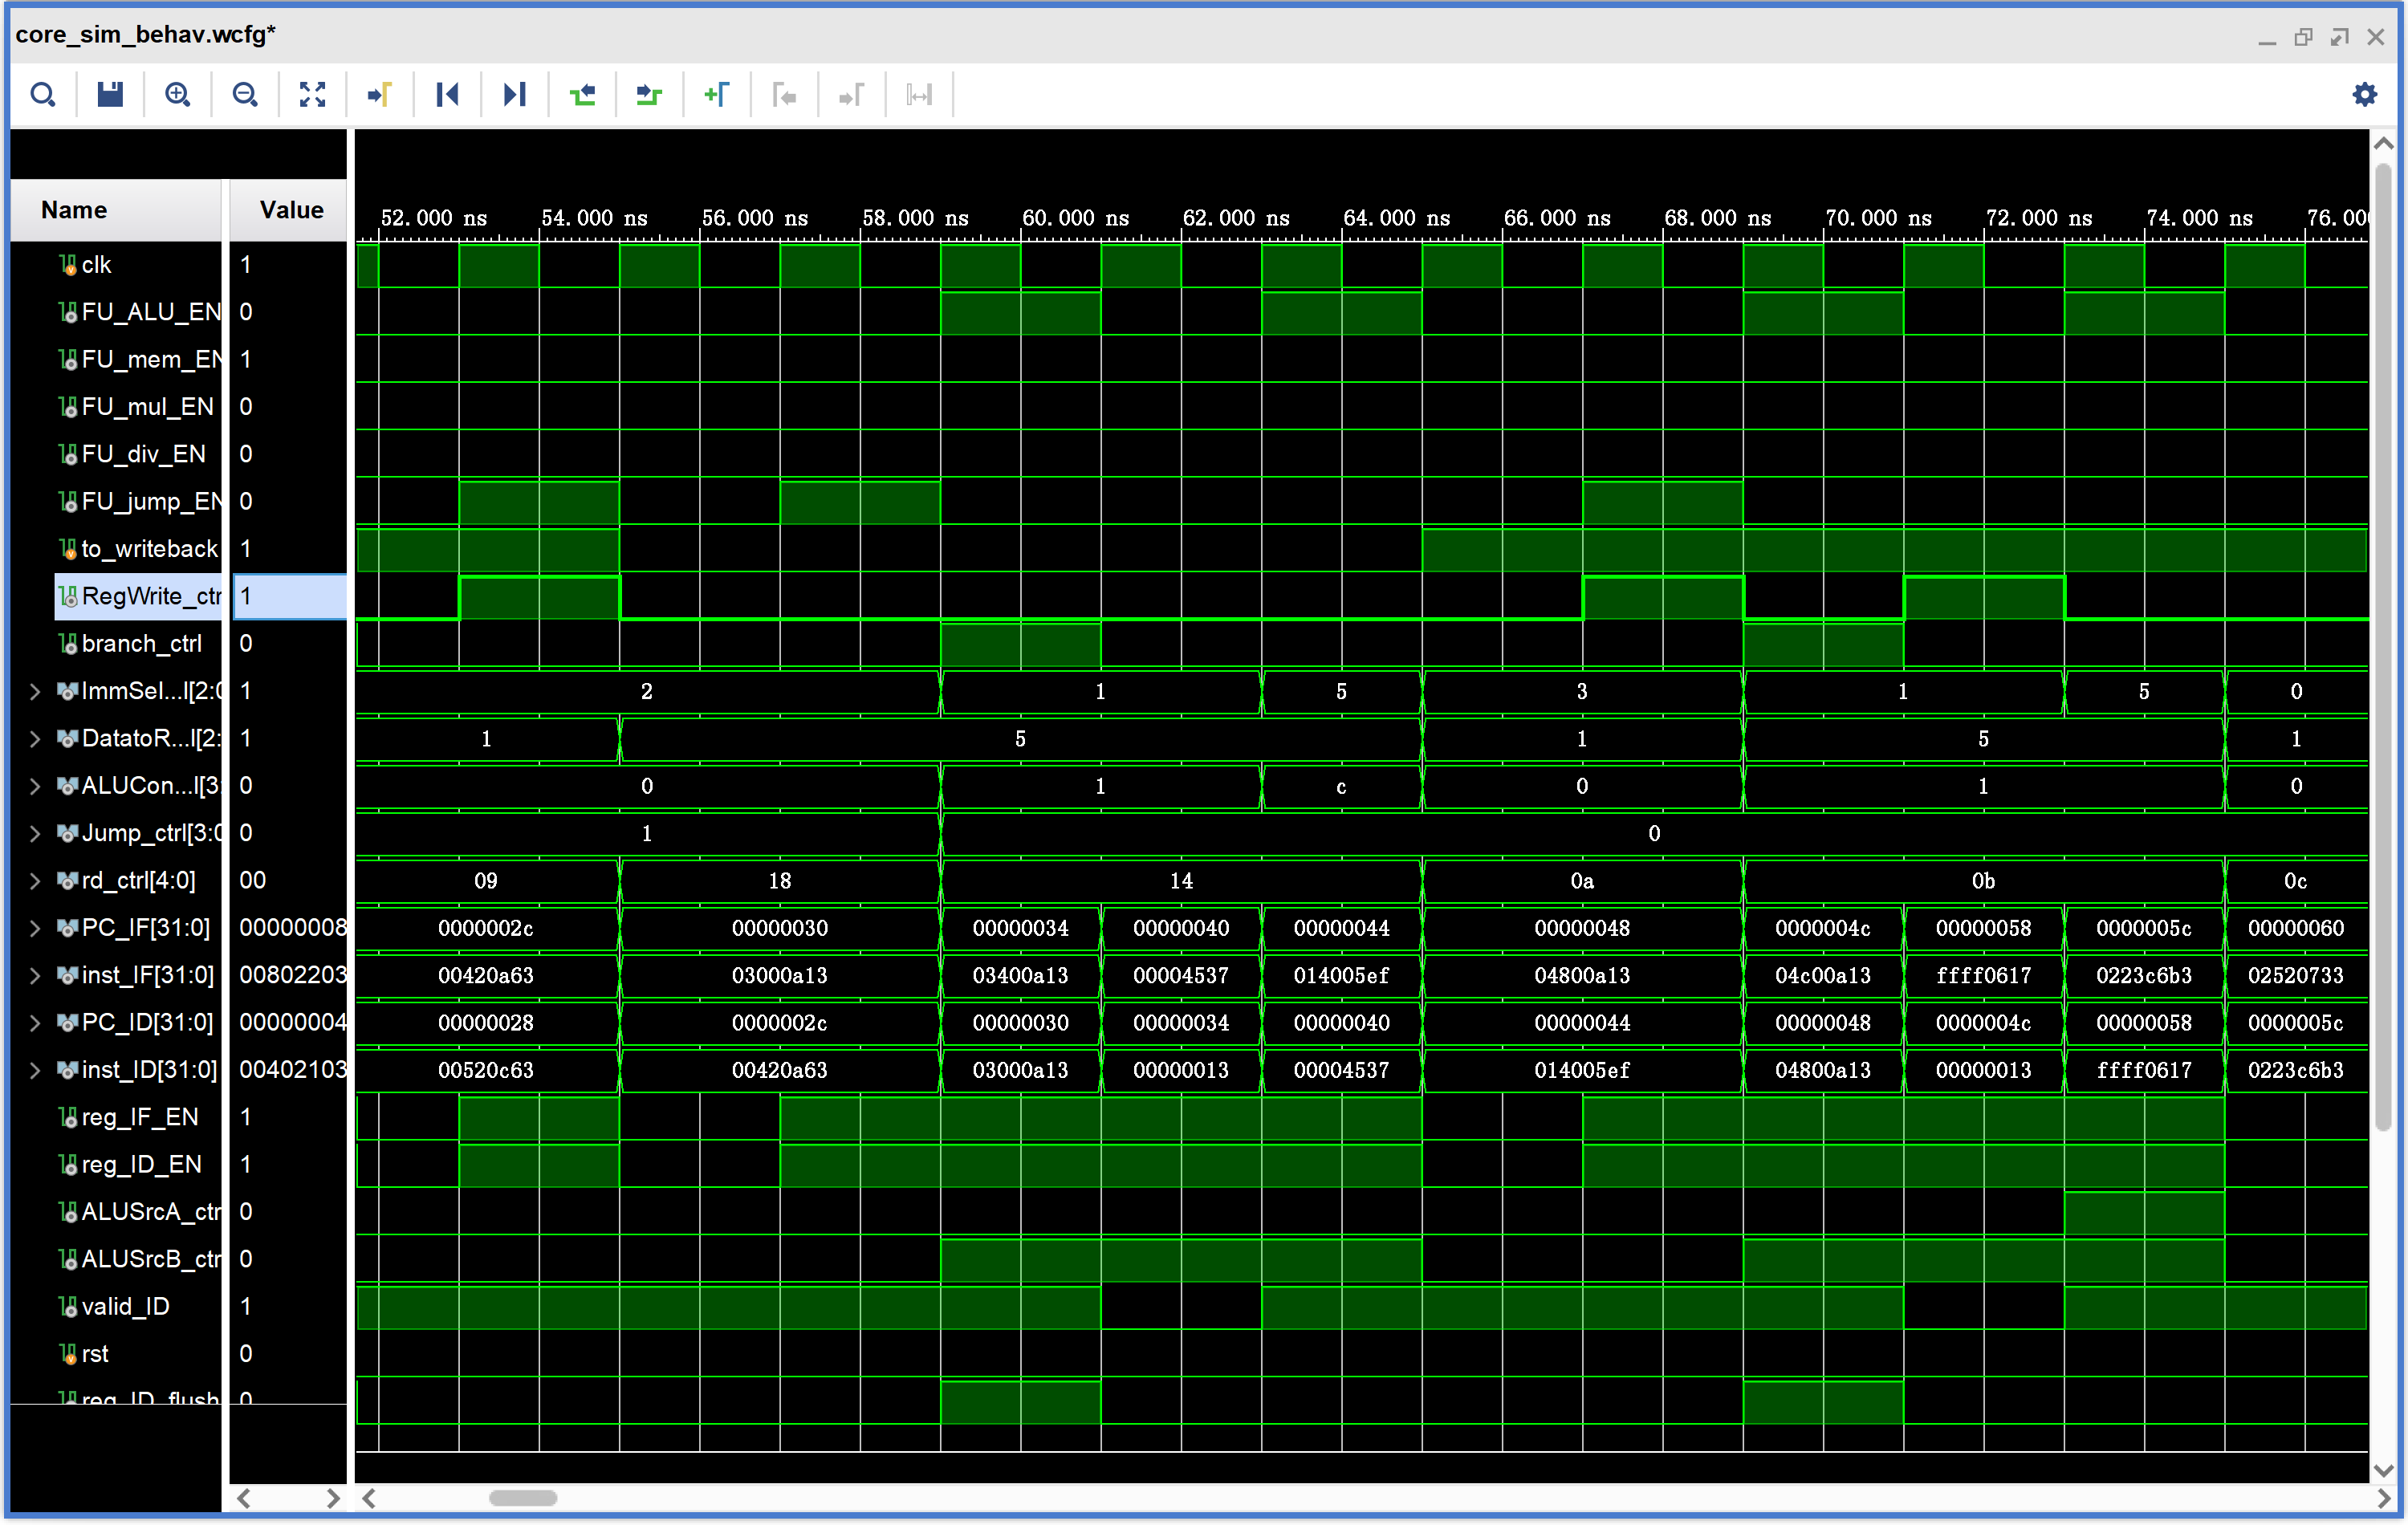
\includegraphics[width=1.0\textwidth]{figs/3.png} %插入图片,[]中设置图片大小,{}中是图片文件名
	\caption{Cache Operation Flow} %最终文档中希望显示的图片标题
	\label{Fig.2} %用于文内引用的标签
\end{figure}
当CPU需要对数据进行操作时,会首先传入read或write bit。CMU接收到信号后首先查看地址是否hit,若hit则直接读或写数据。否则检查需要置换的block是否dirty,若dirty则需要先将当前块写回memory。之后从memory中取数据存入cache,再进行读或写操作。
\subsection{Cache Management State Machine}
CMU的内部结构实际上是一个有限状态机,其有S\_IDLE、S\_PRE\_BACK、S\_BACK、S\_FILL、S\_WAIT等5个状态。
\begin{figure}[H] %H为当前位置,!htb为忽略美学标准,htbp为浮动图形
	\centering %图片居中
	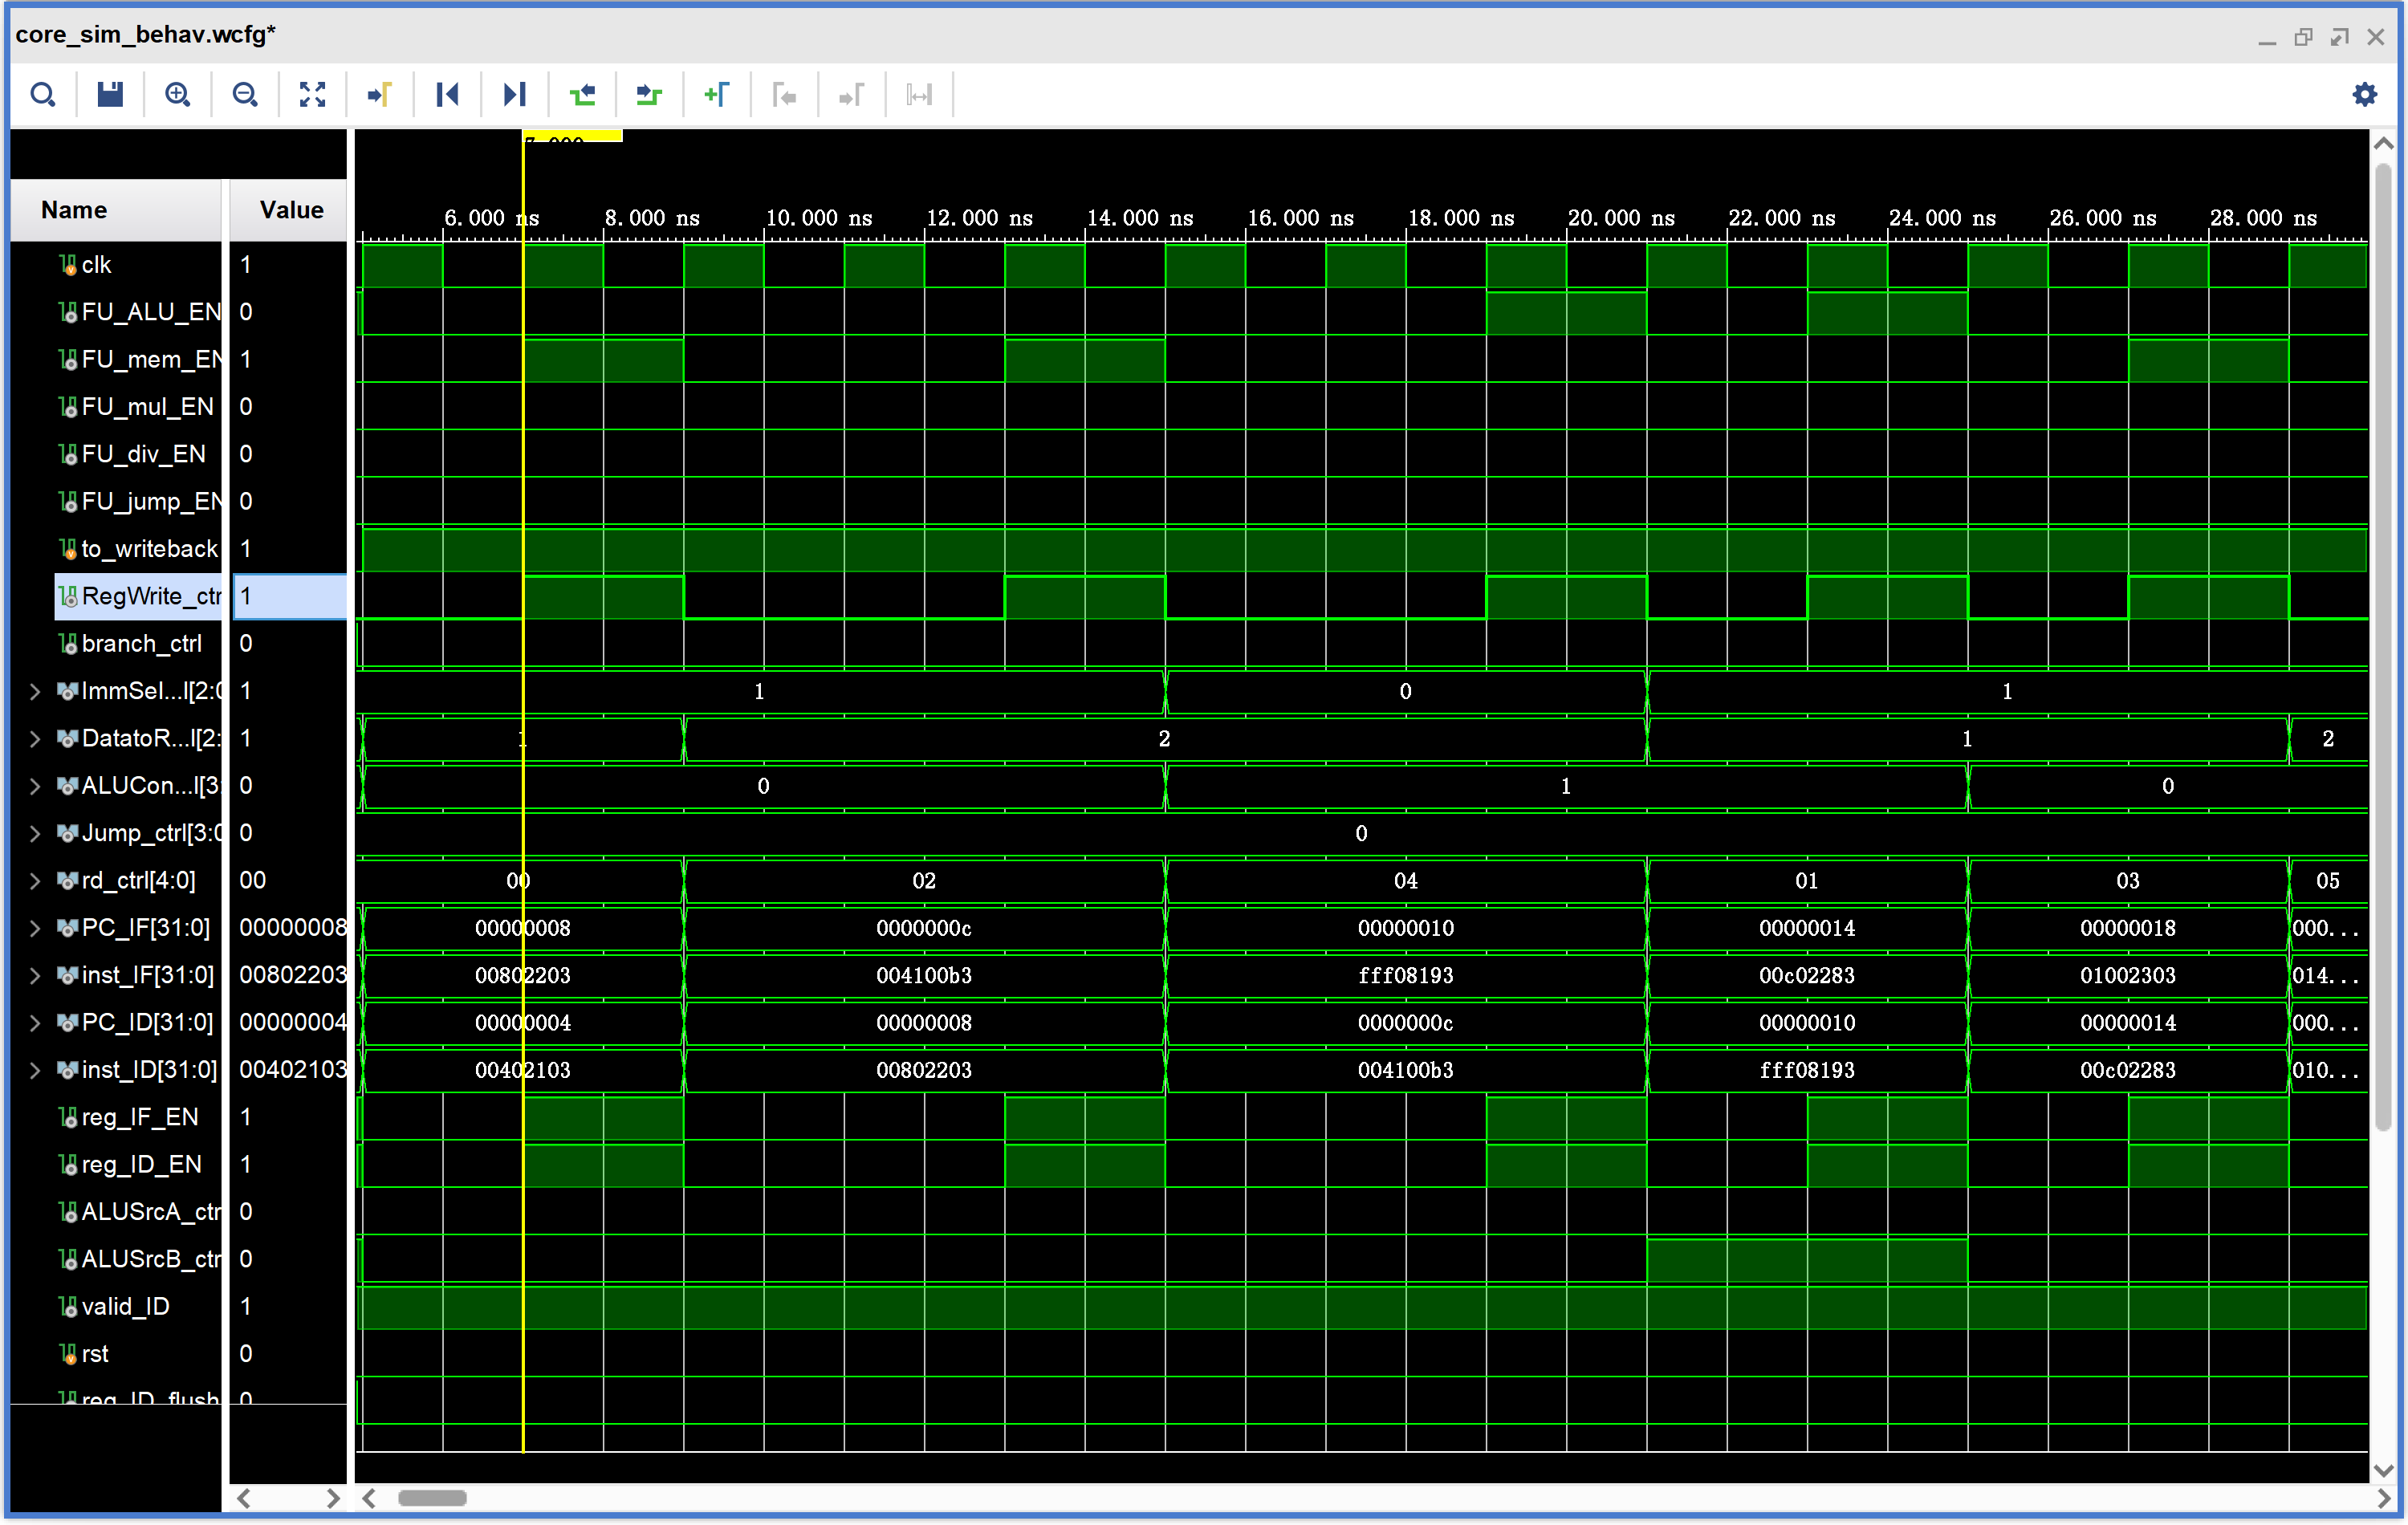
\includegraphics[width=1.0\textwidth]{figs/2.png} %插入图片,[]中设置图片大小,{}中是图片文件名
	\caption{CMU状态机} %最终文档中希望显示的图片标题
	\label{Fig.3} %用于文内引用的标签
\end{figure}
cache操作均发生在当前state的下降沿,memory操作均发生在当前state的上升沿。 每个状态的具体描述如下:
\begin{itemize}
	\item [1.] S\_IDLE:空闲状态,不进行memory操作,cache操作hit的情况下一直处于这个状态。
	\item [2.] S\_PRE\_BACK:为了写回,先进行一次读cache。
	\item [3.] S\_BACK:上升沿将上个状态的数据写回到memory,下降沿从cache读下次需要写回的数据,由计数器控制直到整个cache line全部写回。由于memory设置为4个周期完成读写操作,因此需要等待memory给出ack信号,才能进行状态的改变。
	\item [4.] S\_FILL:上升沿从memory读取数据,下降沿向cache写入数据,由计数器控制直到整个cache line全部写入。与S\_BACK类似,需要等待ack信号。
	\item [5.] S\_WAIT:执行之前由于miss而不能进行的cache操作。
\end{itemize}
\subsection{源代码}
\begin{lstlisting}[language = {verilog}]
module cmu (
	// CPU side
	input clk,
	input rst,
	input [31:0] addr_rw,
	input en_r,
	input en_w,
	input [2:0] u_b_h_w,
	input [31:0] data_w,
	output [31:0] data_r,
	output stall,
	
	// mem side
	output reg mem_cs_o = 0,
	output reg mem_we_o = 0,
	output reg [31:0] mem_addr_o = 0,
	input [31:0] mem_data_i,
	output [31:0] mem_data_o,
	input mem_ack_i,
	
	// debug info
	output [2:0] cmu_state
	);
	
	`include "addr_define.vh"
	
	reg [ADDR_BITS-1:0] cache_addr = 0;
	reg cache_load = 0;
	reg cache_store = 0;
	reg cache_edit = 0;
	reg [2:0] cache_u_b_h_w = 0;
	reg [WORD_BITS-1:0] cache_din = 0;
	wire cache_hit;
	wire [WORD_BITS-1:0] cache_dout;
	wire cache_valid;
	wire cache_dirty;
	wire [TAG_BITS-1:0] cache_tag;
	
	cache CACHE (
	.clk(~clk),
	.rst(rst),
	.addr(cache_addr),
	.load(cache_load),
	.store(cache_store),
	.edit(cache_edit),
	.invalid(1'b0),
	.u_b_h_w(cache_u_b_h_w),
	.din(cache_din),
	.hit(cache_hit),
	.dout(cache_dout),
	.valid(cache_valid),
	.dirty(cache_dirty),
	.tag(cache_tag)
	);
	
	localparam
	S_IDLE = 0,
	S_PRE_BACK = 1,
	S_BACK = 2,
	S_FILL = 3,
	S_WAIT = 4;
	
	reg [2:0]state = 0;
	reg [2:0]next_state = 0;
	reg [ELEMENT_WORDS_WIDTH-1:0]word_count = 0;
	reg [ELEMENT_WORDS_WIDTH-1:0]next_word_count = 0;
	assign cmu_state = state;
	
	always @ (posedge clk) begin
	if (rst) begin
	state <= S_IDLE;
	word_count <= 2'b00;
	end
	else begin
	state <= next_state;
	word_count <= next_word_count;
	end
	end
	
	// state ctrl
	always @ (*) begin
	if (rst) begin
	next_state = S_IDLE;
	next_word_count = 2'b00;
	end
	else begin
	case (state)
	S_IDLE: begin
	if (en_r || en_w) begin
	if (cache_hit)
	next_state = S_IDLE;
	else if (cache_valid && cache_dirty)
	next_state = S_PRE_BACK;
	else
	next_state = S_FILL;
	end
	next_word_count = 2'b00;
	end
	
	S_PRE_BACK: begin
	next_state = S_BACK;
	next_word_count = 2'b00;
	end
	
	S_BACK: begin //?
	if (mem_ack_i && word_count == {ELEMENT_WORDS_WIDTH{1'b1}})    // 2'b11 in default case
	next_state = S_FILL;
	else
	next_state = S_BACK;
	
	if (mem_ack_i)
	next_word_count = word_count + 2'b01; //?
	else
	next_word_count = word_count;
	end
	
	S_FILL: begin
	if (mem_ack_i && word_count == {ELEMENT_WORDS_WIDTH{1'b1}})
	next_state = S_WAIT;
	else
	next_state = S_FILL;
	
	if (mem_ack_i)
	next_word_count = word_count + 2'b01;
	else
	next_word_count = word_count;
	end
	
	S_WAIT: begin
	next_state = S_IDLE;
	next_word_count = 2'b00;
	end
	endcase
	end
	end
	
	// cache ctrl
	always @ (*) begin
	case(state)
	S_IDLE, S_WAIT: begin
	cache_addr = addr_rw;
	cache_load = en_r;
	cache_edit = en_w;
	cache_store = 1'b0;
	cache_u_b_h_w = u_b_h_w;
	cache_din = data_w;
	end
	S_BACK, S_PRE_BACK: begin
	cache_addr = {addr_rw[ADDR_BITS-1:BLOCK_WIDTH], next_word_count, {ELEMENT_WORDS_WIDTH{1'b0}}};
	cache_load = 1'b0;
	cache_edit = 1'b0;
	cache_store = 1'b0;
	cache_u_b_h_w = 3'b010;
	cache_din = 32'b0;
	end
	S_FILL: begin
	cache_addr = {addr_rw[ADDR_BITS-1:BLOCK_WIDTH], word_count, {ELEMENT_WORDS_WIDTH{1'b0}}};
	cache_load = 1'b0;
	cache_edit = 1'b0;
	cache_store = mem_ack_i;
	cache_u_b_h_w = 3'b010;
	cache_din = mem_data_i;
	end
	endcase
	end
	assign data_r = cache_dout;
	
	// mem ctrl
	always @ (*) begin
	case (next_state)
	S_IDLE, S_PRE_BACK, S_WAIT: begin
	mem_cs_o = 1'b0;
	mem_we_o = 1'b0;
	mem_addr_o = 32'b0;
	end
	
	S_BACK: begin
	mem_cs_o = 1'b1;
	mem_we_o = 1'b1;
	mem_addr_o = {cache_tag, addr_rw[ADDR_BITS-TAG_BITS-1:BLOCK_WIDTH], next_word_count, {ELEMENT_WORDS_WIDTH{1'b0}}};
	end
	
	S_FILL: begin
	mem_cs_o = 1'b1;
	mem_we_o = 1'b0;
	mem_addr_o = {addr_rw[ADDR_BITS-1:BLOCK_WIDTH], next_word_count, {ELEMENT_WORDS_WIDTH{1'b0}}};
	end
	endcase
	end
	assign mem_data_o = cache_dout;
	
	//important
	assign stall = (next_state != S_IDLE);
	
endmodule
	
\end{lstlisting}